\chapter{Tips in DL}

重要的一点说明:CNN中的卷积操作其实是信号处理中的相关操作(Correlation Operation)。

\section{Enlarge the FOV}

增加网络的感受野。目前看到的主要方法如下:

\begin{itemize}
\item CRFs\cite{marvin2018crf}
\item Global Graph-reasoning module\cite{chen18iterative}
\item Pooling
\item Dilated conv\cite{YuKoltun2016}
\item 
\end{itemize}


\section{Upsampling}

在卷积以及Pooling之后保持分辨率。目前看到的主要方法如下:

\begin{itemize}
\item Padding
\item Deconvolution
\item Uppooling
\item Bilinear
\item 
\end{itemize}


\section{Multiscale Ability}

在目标检测(Object Detection)中加入多尺度信息。记得的有以下几个方法:

\begin{itemize}
\item Pyramid Network
\item Stacked CNN ?
\item 
\end{itemize}


\section{Dilated Convolution}

主要原理如下。

\begin{figure}[!hbtp]
\centering
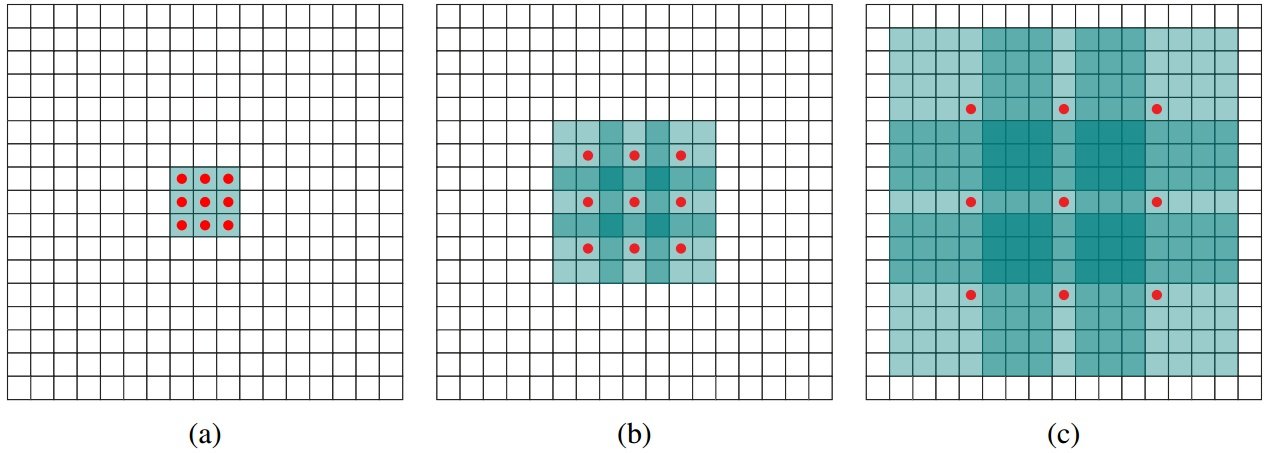
\includegraphics[width=0.75\textwidth]{DLTips/DilatedConv1}
\caption{Dilated Convolution示意图}
\label{DilatedConv1}
\end{figure}

{\bfseries 注意,下文提到的N-Dilated Conv中的$N={1, 2, 3, \ldots}$是指图中相邻红点之间的间隔。}

图\ref{DilatedConv1}中,(a)图对应3x3的1-dilated conv,和普通的卷积操作一样,(b)图对应3x3的2-dilated conv,实际的卷积kernel size还是3x3,但是空洞为1,也就是对于一个7x7的图像patch,只有9个红色的点和3x3的kernel发生卷积操作,其余的点略过。也可以理解为kernel的size为7x7,但是只有图中的9个点的权重不为0,其余都为0。 可以看到虽然kernel size只有3x3,但是这个卷积的感受野已经增大到了7x7{\bfseries(如果考虑到这个2-dilated conv的前一层是一个1-dilated conv的话,那么每个红点就是1-dilated的卷积输出,所以感受野为3x3,所以1-dilated和2-dilated合起来就能达到7x7的conv)},(c)图是4-dilated conv操作,同理跟在两个1-dilated和2-dilated conv的后面,能达到15x15的感受野。对比传统的conv操作,3层3x3的卷积加起来,stride为1的话,只能达到(kernel-1)*layer+1=7的感受野,也就是和层数layer成线性关系,而dilated conv的感受野是指数级的增长。

Dilated的好处是不做Pooling算是信息的情况下,加大了感受野,让每个卷积核输出都包含较大范围的信息。在图像需要全局信息或者语音文本需要较长的Sequence信息依赖的问题中,都能很好的应用Dilated Convolution, 比如图像分割、语音合成WaveNet、机器翻译ByteNet。

WaveNet的例子。
\begin{figure}[!hbtp]
\centering
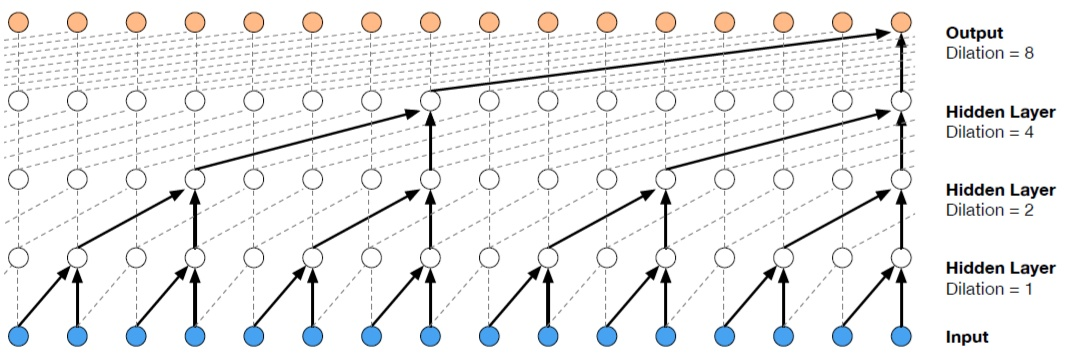
\includegraphics[width=0.75\textwidth]{DLTips/WaveNet1}
\caption{Dilated Convolution在WaveNet中的应用示意图}
\label{WaveNet1}
\end{figure}

参考文献:\href{https://www.zhihu.com/search?type=content\&q=dilated\%20CNN}{Dilated Conv 知乎}

\section{Deconvolutional Network}

务必看\textbf{补充}部分的内容!

参考文献:\href{https://www.zhihu.com/question/43609045/answer/132235276}{Deconvolution Networks}

可能应用的领域:Visualization, Pixel-wise Prediction, Unsupervised Learning, Image Generation.

大致可分为以下几个方面:
\begin{itemize}
\item Unsupervised Learning 

其实是 Covolutional Sparse Coding. 这里的Deconv只是观念上和传统的Conv反向,传统的conv是从图片生成feature map,而deconv是用unsupervised的方法找到一组kernel和feature map,让它们重建图片。

\item CNN Visualization

通过deconv将CNN中conv得到的feature map还原到像素空间,以观察特定的feature map对哪些pattern的图片敏感,这里的deconv其实不是conv的可逆运算,只是conv的transpose,所以tensorflow里一般取名叫transpose\_conv。

\item Upsampling

在pixel-wise prediction比如image segmentation[4]以及image generation[5]中,由于需要做原始图片尺寸空间的预测,而卷积由于stride往往会降低图片size, 所以往往需要通过upsampling的方法来还原到原始图片尺寸,deconv就充当了一个upsampling的角色。

\end{itemize}

下面主要介绍这三个方面的论文。

\subsection{Convolutional Spare Coding}

{\bfseries 第一篇:Deconvolutional Netwoks}

主要用于学习图片的中低层级的特征表示,属于Unspervised Feature Learning。

更多内容参考本小节的参考文献。

\subsection{CNN可视化}
ZF-Net中利用Deconv来做可视化,它是将CNN学习到的Feature Map的卷积核,取转置,将图片特征从Feature Map空间转化到Pixel空间,用于发现哪些Pixel激活了特定的Feature Map,达到分析理解CNN的目的。


\subsection{Upsampling}
用于FCN\cite{Fcn2014}和DCGAN。

\subsection{补充}

{\bfseries 一个非常好的可以看到多种卷积操作动作图的资源:}\href{https://github.com/vdumoulin/conv_arithmetic}{Convolution Arithmetic Github}


上面的东西还是没有说明白Deconvolution到底是怎么回事啊。

\begin{quote}
实际使用中,反卷积会引起棋盘状的Artifacts。所以要采用上采样卷积层。
\end{quote}
上面这句话是什么意思?

\subsection{Deconvolution与Upsample的区别}

参考文献:\href{https://www.zhihu.com/question/63890195}{Caffe中的Deconvolution和Upsample区别-知乎}

高票回答:

Deconvolution

\begin{figure}[!htbp]
\centering
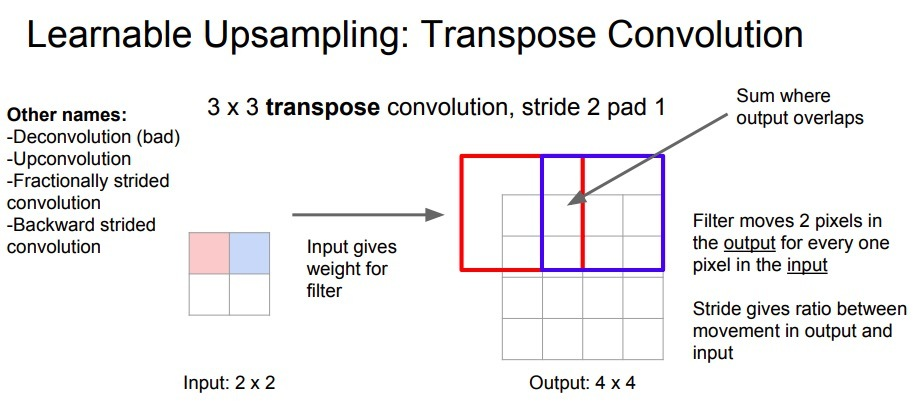
\includegraphics[width=0.75\textwidth]{DLTips/Deconvolution0.jpg}
\caption{Transpose Convolution过程示意图}
\label{Deconvolution0}
\end{figure}

Input pixel * filter = output window,不同output window重合的部分使用sum叠加处理。

这一解释和caffe的定义保持一致,caffe中定义解释过来就是:“DeconvolutionLayer 逐像素地将输入值乘上一个filter,并将结果输出windows叠加起来”

Convolve the input with a bank of learned filters, and (optionally) add biases, treating filters and convolution parameters in the opposite sense as ConvolutionLayer.ConvolutionLayer computes each output value by dotting an input window with a filter; DeconvolutionLayer multiplies each input value by a filter elementwise, and sums over the resulting output windows. In other words, DeconvolutionLayer is ConvolutionLayer with the forward and backward passes reversed. DeconvolutionLayer reuses ConvolutionParameter for its parameters, but they take the opposite sense as in ConvolutionLayer (so padding is removed from the output rather than added to the input, and stride results in upsampling rather than downsampling).

Upsampling

该层权重通过BilinearFiller初始化,因此当学习率为0时,权重在训练过程中保持初始值不变,一一直作为bilinear resize的作用。

\lstset{language=Python, caption={Bilinear filter initializer in MXNet}}
\begin{lstlisting}
class Bilinear(Initializer)
"""Initialize weight for upsampling layers."""
def __init__(self):
    super(Bilinear, self).__init__()
def _init_weight(self, _, arr):
    weight = np.zeros(np.prod(arr.shape), dtype='float32')
    shape = arr.shape
    f = np.ceil(shape[3] / 2.)
    c = (2 * f - 1 - f % 2) / (2. * f)
    for i in range(np.prod(shape)):
        x = i % shape[3]
        y = (i / shape[3]) % shape[2]
        weight[i] = (1 - abs(x / f - c)) * (1 - abs(y / f - c))
    arr[:] = weight.reshape(shape)
\end{lstlisting}

James Liu的回答:

\begin{itemize}
\item \textbf{Deconvolution}

上采样就是把$[W,H]$大小的feature map $F_{W,H}$扩大为$[nW,nH]$尺寸大小的$\hat{F}_{nW,nH}$,其中$n$为上采样倍数。那么可以很容易的想到我们可以在扩大的feature map $\hat{F}$上每隔$n$个位置填补原F中对应位置的值。

但是剩余的那些位置怎么办呢?deconv操作是把剩余位置填0,然后这个大feature map过一个conv。

\textbf{所以}:Deconv = 扩大 + 填0 + Convolution

\item \textbf{Upsampling}

插值上采样 = 扩大 + 插值

\end{itemize}

\subsubsection{理解深度学习中的Deconvolution Networks}

参考文献:\href{https://www.zhihu.com/question/43609045}{理解深度学习中的Deconvolution Networks - 知乎}


逆卷积(Deconvolution)比较容易引起误会,转置卷积(Transposed Convolution)是一个更为合适的叫法.

\begin{figure}[!hbtp]
\centering
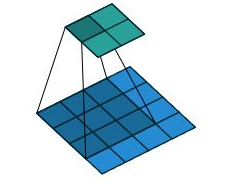
\includegraphics[width=0.5\textwidth]{DLTips/Deconvolution1.png}
\caption{一个例子,用于卷积操作说明}
\label{Deconvolution1}
\end{figure}
输入矩阵可展开为16维向量,记作x

输出矩阵可展开为4维向量,记作y

卷积运算可表示为y = Cx

不难想象C其实就是如下的稀疏阵
\begin{figure}[!htbp]
\centering
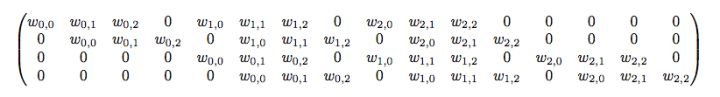
\includegraphics[width=0.5\textwidth]{DLTips/Deconvolution2.jpg}
\caption{卷积操作时的矩阵形式}
\label{Deconvolution2}
\end{figure}

那么当反向传播时又会如何呢?首先我们已经有从更深层的网络中得到的$\frac{\partial Loss}{\partial y}$.

\begin{displaymath}
\frac{\partial{Loss}}{\partial{x_j}} = \sum_{i}\frac{\partial{Loss}}{\partial y_i} \frac{\partial y_i}{\partial{x_j}} = \sum_{i} \frac{\partial{Loss}}{\partial y_i} C_{i, j} = \frac{\partial{Loss}}{y} \cdot C_{*, j} = C_{*, j}^T \frac{\partial{Loss}}{\partial y}
\end{displaymath}

回想第一句话,你猜的没错,所谓逆卷积其实就是正向时左乘$C^T$,而反向时左乘$(C^T)^T$,即C的运算。

为什么CS321n里面说要使用Convolution Transpose而不是Deconvolution呢:

反卷积的数学含义,通过反卷积可以将通过卷积的输出信号,完全还原输入信号。

而事实是,转置卷积只能还原shape大小,不能还原value.

\section{Dilated Network与Deconv Network之间的区别}
Dilated Convolution主要用于增加感受野,而不是Upsampling;Deconv Network主要用于Upsample,即增加图像分辨率。

对于标准的$k \times k$的卷及操作,stride为$s$,分为一下几种情况:
\begin{itemize}
\item $s > 1$

即卷积的同时做了降采样,输入Feature Map的分辨率\footnote{分辨率是指像素的多少,而尺度是指模糊程度的大小,即Gaussian Filter中的方差$\delta$}下降。但这一般也会增加感受野。

\item $s = 1$

普通的步长为1的卷积,输入与输出分辨率相同。

\item $\mathbf{0 < s < 1}$

Fractionally strided convolution.相当于图像做upsampling。比如$s=0.5$时,意味着图像像素之间padding一个空白的像素(像素值为0)后,stride改为1进行卷积,达到一次卷积看到的空间范围变大的目的。

\end{itemize}

\section{目标检测中的mAP的含义}

\begin{itemize}
\item 对于类别C,在一张图像上

首先计算C在一张图像上的精度。

\begin{displaymath}
\label{PrecisionC1}
Precision_C = \frac{N(TP)_C}{N(Total)_C}
\end{displaymath}
其中,$Precision_C$为类别C在一张图像上的精度。$N(TP)_C$为算法检测正确(True Positive)的$C$的个数,检测是否正确按照$IoU > 0.5$算,同理,$T(Total)_C$为这一张图像所有$C$类的个数。所以则一步,仅涉及一个类别$C$以及一张图像。

\item 对于类别C,在多张图像上

这一步计算的是类别$C$的$AP$指数。

\begin{displaymath}
\label{PrecisionC2}
AveragePrecision_C = \frac{\sum Precision_C}{N(TotalImage)_C}
\end{displaymath}
其中,$AveragePrecision_C$是类别$C$的$AP$指数,$Precision_C$为上文计算得到的类别$C$的在一张图像上的精度,然后对所有包含类别$C$的图像上的$C$的精度$Precision_C$求和;$N(TotalImage)_C$为包含类别$C$的图像的数量,也对应于分子中求和所涉及的图像。

\item 在整个数据集上,多个类别

$mAP$在上一步的计算结果的基础上,计算所有类别的$AP$和 / 总的类别数。

\begin{displaymath}
\label{PrecisionC3}
meanAveragePrecision = \frac{\sum_{C} AveragePrecision_C}{N(Class)}
\end{displaymath}
也就是相当于计算所有类别的$\mathbf{AP}$的平均值,是对应于类别总数的平均值。

\end{itemize}

参考文献:\href{https://www.zhihu.com/question/53405779}{知乎文章}

\section{统计学习方法}

一个比较好的总结:\href{http://kubicode.me/2015/08/16/Machine%20Learning/Algorithm-Summary-for-Interview/#SVM%E3%80%81SMO}{机器学习常见算法个人总结}


\section{Distillation Module}
文献来源:\cite{Xu2018PADNet}\cite{Mehta2018OD200}

在\cite{Xu2018PADNet}中,同时完成深度估计以及场景解析两个任务。

Distillation Module的目的:
\begin{itemize}
\item Deep-model distilation modules fuses information from the intermediate predictions for each specific final task\cite{Xu2018PADNet}.高效的利用中间任务的信息互补。文章\cite{Xu2018PADNet}提出的三种不同的实现方式如图\ref{ThreeDistillationModules1}所示。

\begin{figure}[!hbtp]
\centering
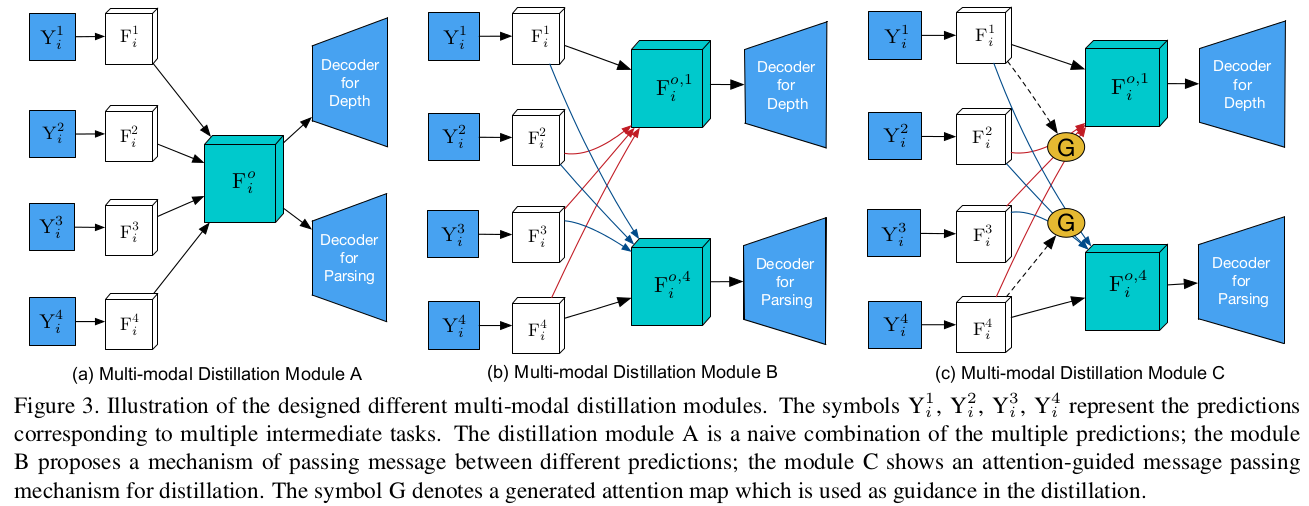
\includegraphics[width=0.75\textwidth]{DLTips/ThreeDistillationModules1.png}
\caption{三种不同的Distillation Module}
\label{ThreeDistillationModules1}
\end{figure}

\item Distillation loss function\cite{Mehta2018OD200}

利用Distillation帮助将Teacher Network(精度更高)的知识迁移到的Student Network.

\end{itemize}

\subsection{Knowledge Distillation}

\subsubsection{什么是Distilling the knowledge}

一句话总结,就是用teacher network的输出作为soft label来训练一个student network.

\subsubsection{Disilling the knowledge in a Neural Network}

\begin{displaymath}
q_i = \frac{exp(z_i/T)}{\sum_{j}exp(z_j/T)}
\end{displaymath}

其实就是一个Softmax,值得注意的是$T$是Temperature,$T$越大,概率分布就越Soft。在训练Student Network时,该概率分布就是Student Network的soft label.

Student Network 的训练策略:
\begin{itemize}
\item 先用Teacher Network的概率分布训练
\item 再用Real Label训练
\end{itemize}

\subsection{Recurrent Knowledge Distillation \cite{Silvia2018Recurrent}}

\section{光流估计中的Average end-point error}

貌似就是类似于均方误差类似。具体定义还没查到。

\section{CNN中的卷及方式汇总}

参考文献:\href{https://zhuanlan.zhihu.com/p/29367273}{CNN中的卷积方式2017.9-知乎}

\subsection{Inception}

\begin{figure}[!htbp]
\centering
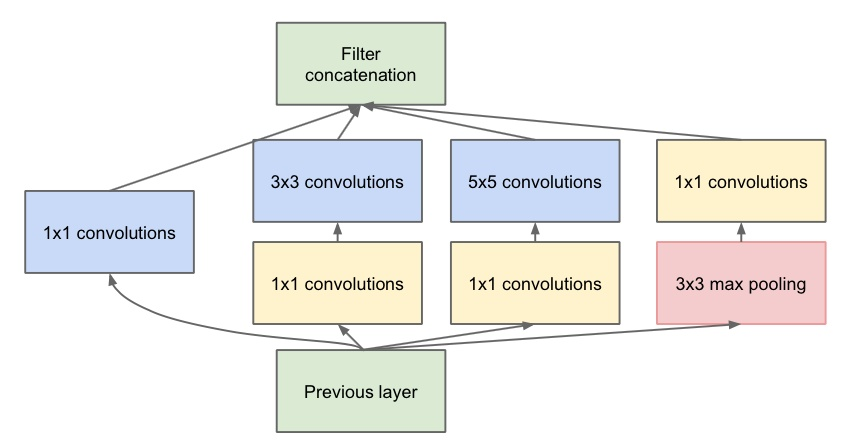
\includegraphics[width=0.9\textwidth]{DLTips/Inception0.jpg}
\caption{Inception卷积结构}
\label{Inception0}
\end{figure}
如图\ref{Inception0}所示。
主要思想是,融合Network in Network的思想来增加隐层提升非线性表达的思想。先用1*1的卷积映射到隐空间,再在隐空间做卷积操作。同时考虑多尺度,在单层Inception中,用多个大小不同的卷积核做卷积,然后把结果Concat起来。

代表模型:
\begin{itemize}
\item Inception-V1

就是把图\ref{Inception0}中的结构进行Stack,GoogLeNet?

\item Inception-V2

加入了Batch Normalization正则,去除了5*5卷积,用两个3*3卷积代替

\item Inception-V3

7 × 7卷积被拆分成7 * 1 + 1 * 7, 可分离卷积?

\item Inception-V4

加入了残差结构。

\end{itemize}

\subsection{空洞卷积, Dilation}

Dilation卷积,通常译作空洞卷积或者卷积核膨胀操作,它是解决pixel-wise输出模型的一种常用的卷积方式。一种普遍的认识是,pooling下采样操作导致的信息丢失是不可逆的,通常的分类识别模型,只需要预测每一类的概率,所以我们不需要考虑pooling会导致损失图像细节信息的问题,但是做像素级的预测时(譬如语义分割),就要考虑到这个问题了。

所以就要有一种卷积代替pooling的作用(成倍的增加感受野),而空洞卷积就是为了做这个的。通过卷积核插“0”的方式,它可以比普通的卷积获得更大的感受野。

所以,本意是为了增加感受野。

应用:
\begin{itemize}
\item FCN
\item WaveNet
\end{itemize}

\subsection{深度可分离卷积, Depthwise Separable Convolution}

是Incepion的延续。

\begin{figure}[!htbp]
\centering
\subfigure[简化的Inception]{\label{Inception1}
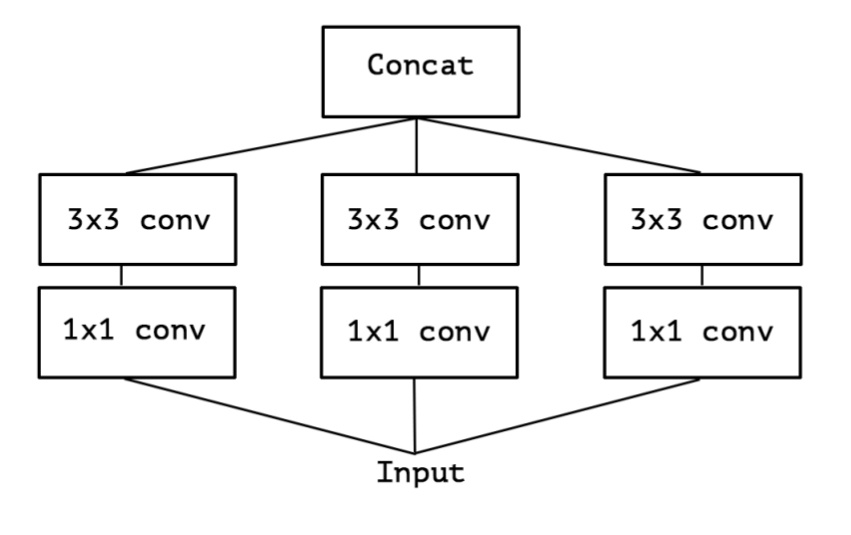
\includegraphics[width=0.95\textwidth]{DLTips/Inception1.jpg}}
\\
\subfigure[Depthwise Separable Convolution的示意图, 可以看出来,与Inception很像。]{\label{DepthwiseSeparable0}
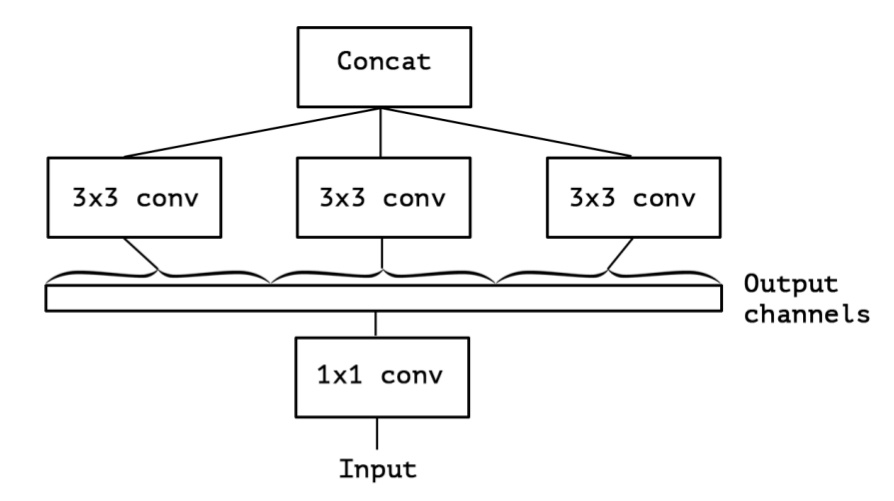
\includegraphics[width=0.95\textwidth]{DLTips/DepthwiseSeparable0.jpg}}
\caption{Inception结构与Depthwise Separable Convolution结构对比}
\label{InceptionAndDepthwise0}
\end{figure}

如图\ref{InceptionAndDepthwise0}所示,我们又可以看做,把一整个输入做1*1卷积,然后切成三段,分别3*3卷积后相连。注意的是,在三个不同的卷积时,是对Channel进行分组进行3*3卷积。

OK,现在我们想,如果不是分成三段,而是分成5段或者更多,那模型的表达能力是不是更强呢?于是我们就切更多段,切到不能再切了,正好是Output channels的数量(极限版本, 图\ref{DepthwiseSeparable1}):

\begin{figure}[!htbp]
\centering
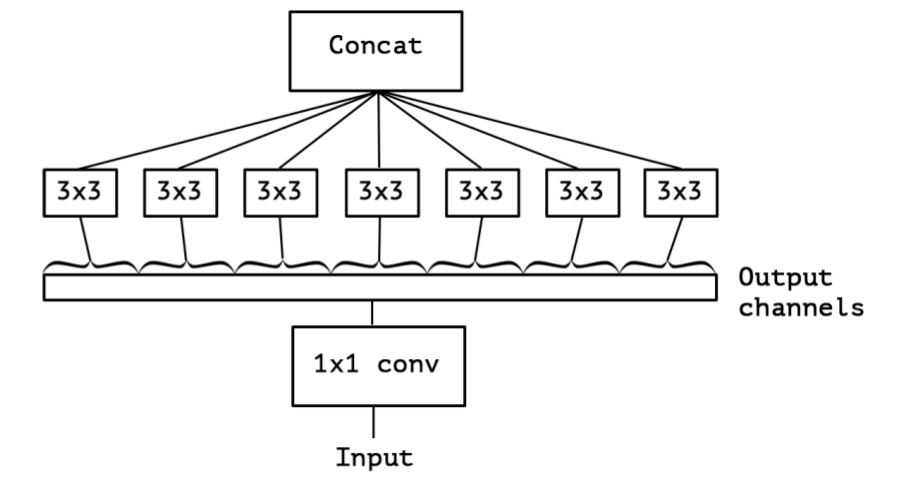
\includegraphics[width=0.75\textwidth]{DLTips/DepthwiseSeparable1.jpg}
\caption{Channel分组的极限版本}
\label{DepthwiseSeparable1}
\end{figure}

于是,就有了深度卷积(depthwise convolution),深度卷积是对输入的每一个channel独立的用对应channel的所有卷积核去卷积,假设卷积核的shape是[filter\_height, filter\_width, in\_channels, channel\_multiplier],那么每个in\_channel会输出channel\_multiplier那么多个通道,最后的feature map就会有in\_channels * channel\_multiplier个通道了。反观普通的卷积,输出的feature map一般就只有channel\_multiplier那么多个通道。

也就是说,对于每一个Channel, 都用不同的多个卷积核进行卷积,具体的是Channel\_multiplier个不同的卷积核。

既然叫深度可分离卷积,光做depthwise convolution肯定是不够的,原文在深度卷积后面又加了pointwise convolution,这个pointwise convolution就是1*1的卷积,可以看做是对那么多分离的通道做了个融合。

这两个过程合起来,就称为Depthwise Separable Convolution了。

应用:
\begin{itemize}
\item Xception
\end{itemize}

\subsection{可变性卷积}

可形变卷积的思想很巧妙:它认为规则形状的卷积核(比如一般用的正方形3*3卷积)可能会限制特征的提取,如果赋予卷积核形变的特性,让网络根据label反传下来的误差自动的调整卷积核的形状,适应网络重点关注的感兴趣的区域,就可以提取更好的特征。

如图\ref{DeformableConv0}:网络会根据原位置(a),学习一个offset偏移量,得到新的卷积核(b)(c)(d),那么一些特殊情况就会成为这个更泛化的模型的特例,例如图(c)表示从不同尺度物体的识别,图(d)表示旋转物体的识别。

\begin{figure}[!htbp]
\centering
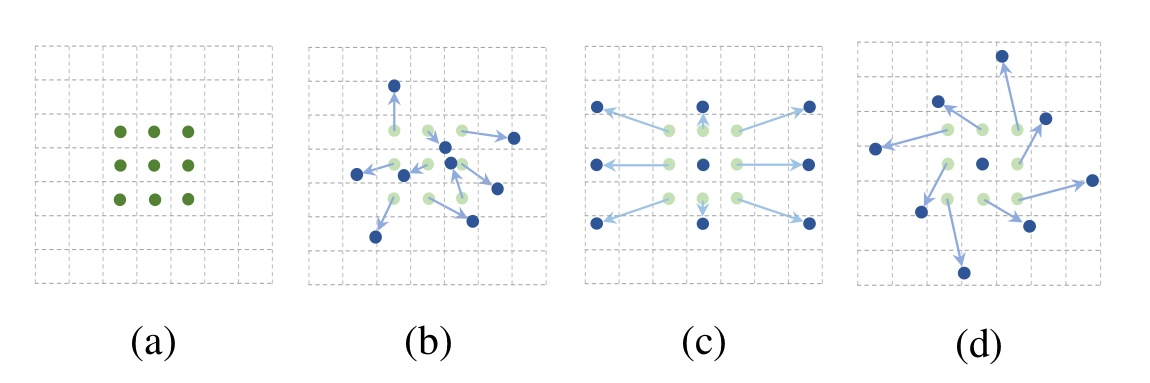
\includegraphics[width=0.95\textwidth]{DLTips/DeformableConv0.jpg}
\caption{Deformable Convolution示意图}
\label{DeformableConv0}
\end{figure}

具体实现如下。

%图\ref{DeformableConv1}中包含两处卷积,第一处是获取offsets的卷积,即我们对input feature map做卷积,得到一个输出(offset field),然后再在这个输出上取对应位置的一组值作为offsets。假设input feature map的shape为[batch,height,width,channels],我们指定输出通道变成两倍,卷积得到的offset field就是[batch,height,width,2×channels],为什么指定通道变成两倍呢?因为我们需要在这个offset field里面取一组卷积核的offsets,而一个offset肯定不能一个值就表示的,最少也要用两个值(x方向上的偏移和y方向上的偏移)所以,如果我们的卷积核是3*3,那意味着我们需要3*3个offsets,一共需要2*3*3个值,取完了这些值,就可以顺利使卷积核形变了。第二处就是使用变形的卷积核来卷积,这个比较常规。(这里还有一个用双线性插值的方法获取某一卷积形变后位置的输入的过程)

图\ref{DeformableConv1}中包含两处卷积。第一处是绿色的获取Offsets的卷积,即图中上方部分,这一处的输入是Input feature map,得到一个输出(Offset Feild), 然后再在这个输出上取一个卷积核大小的切片,作为卷积核对应位置的Offset。若Input Feature的尺寸为:$Batch, height, width, channels$, 其中,Batch表示批数, Channel表示输入的通道数,然后输出通道变为两倍,卷积得到的Offset Field就是$Batch, height, width, 2 *  channels$,那么为什么会翻倍呢, 也就是图中上半部分中的2N是什么意思呢?首先要确定一个卷积核的Offset,需要在不同的方向上单独确定,比如X, Y方向,所以就变成二倍了。在实际进行Deformable时,首先从Offset Field中对应位置上取一个对应卷积核的切片,如果卷积核是3 * 3,那么我们在两个方向都取一个3 * 3的切片,代表来年各个方向的Offset,然后就完成卷积核形变了。

第二处的卷积,是图中下方的表示,就是一个常规的卷积运算,只不过卷积核是经过上述Offset之后的变形卷积核。这里还有一个用双线性插值的方法来获取某一卷积形变后位置的输入的过程。

\begin{figure}[!htbp]
\centering
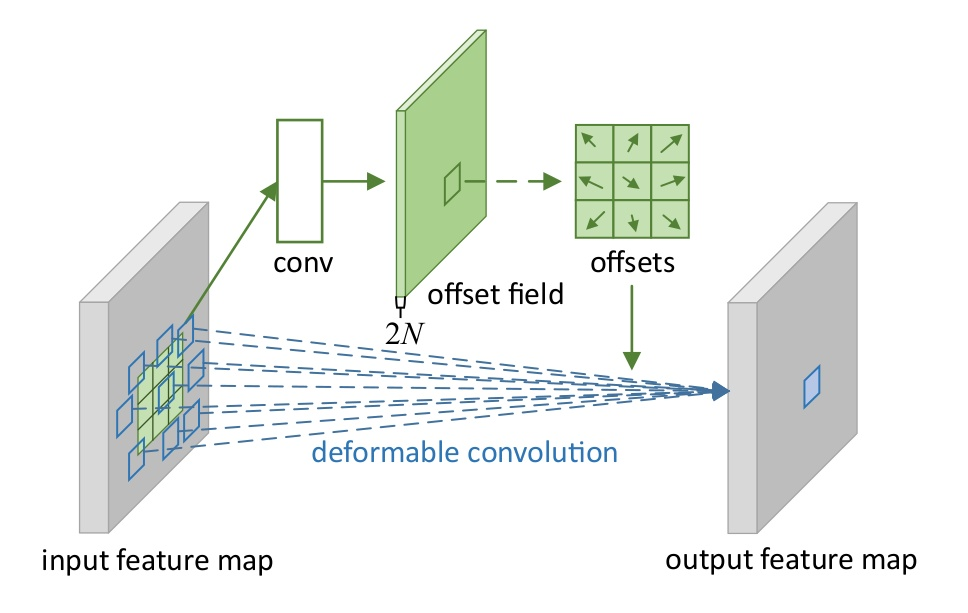
\includegraphics[width=0.95\textwidth]{DLTips/DeformableConv1.jpg}
\caption{Deformable Convolution的实现示意图}
\label{DeformableConv1}
\end{figure}

应用:
\begin{itemize}
\item Deformable Convolutional Networks
\end{itemize}

可能 会跟目标检测、跟踪相结合。

\subsection{特征重标定卷积}

在ImageNet2017比赛中,冠军模型SENet的核心模块,被称为"Squeeze-and-Excitation", 知乎的作者把它就先成为特征重标定卷积了。

和前面的不同,本文提出的算法的出发点在于改进特征为度,包括卷积核的数量等。现在一个卷积层中,还不是整个神经网络,有数以千计的卷积核,而且我们知道每一种卷积核对应提取一种特征,但得到这么多的特征,肯定有一些是更重要的,有一些是不那么重要的。所以本文的方法是通过学习方式来自动获取每个特征通道的重要程度,然后按照计算出来的重要程度去提升有用的特征并抑制对当前任务用处不大的特征。

\begin{figure}[!htbp]
\centering
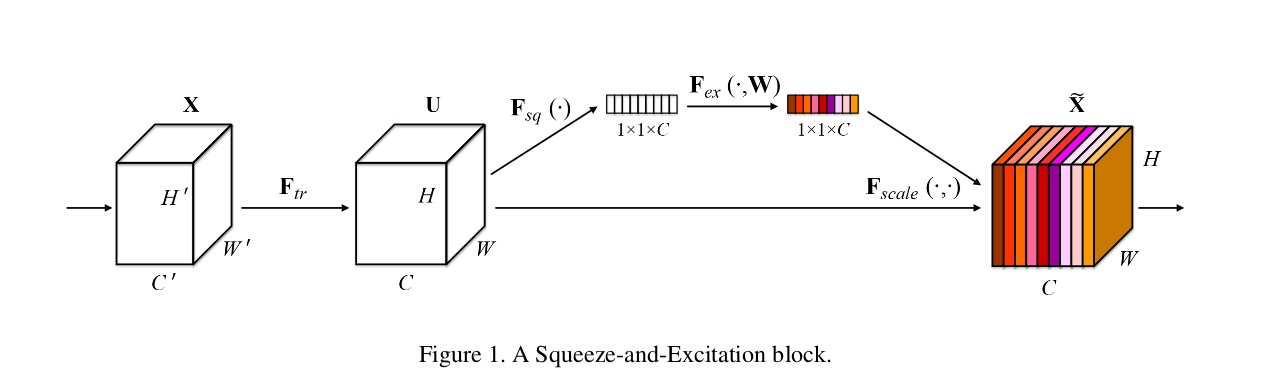
\includegraphics[width=0.9\textwidth]{DLTips/SENetConv0.jpg}
\caption{Squeeze-and-Excitation Block示意图}
\label{SENetConv0}
\end{figure}

虽然听上去很复杂,但实现起来却比较简单?步骤如下:
\begin{itemize}
\item 首先对输入$X$做常规的卷积$F_{tr}$,得到一个Output Feature Map ($U$),它的大小为$C, H, W$, 文章的作者认为,得到的这个Output是非常混乱的。
\item 为了得到这些Feature Maps(共$C$个)的重要程度,直接对这些Feature Map做一个Global Average Pooling\footnote{这里还涉及到一个额外的东西,如果你了解卷积,你就会发现一旦某一特征经常被激活,那么Global Average Pooling计算出来的值会比较大,说明它对结果的影响也比较大,反之越小的值,对结果的影响就越小。}, 然后就得到一个长度为$C$的向量,注意是向量了! 在图\ref{SENetConv0}中表现就是由$U$经操作$F_{sq}(\cdot)$得到$1 \times 1 \times C$的过程。

\item 然后我们对这个向量加两个FC层,做非线性映射,这俩FC层的参数,也就是网络需要额外学习的参数。对应图中$F_{ex}(\cdot, W)$操作。

\item 最后输出的向量,我们可以看做特征的重要性程度,然后与feature map对应channel相乘就得到特征有序的feature map了。对应图中$F_{scale}(\cdot, \cdot)$操作。
\end{itemize}

应用:
\begin{itemize}
\item Squeeze-and-Excitation Networks
\item 另外它还可以和几个主流网络结构结合起来一起用,比如Inception和Res。图\ref{SENetConv1}所示。
\end{itemize}

\begin{figure}[!htbp]
\centering
\subfigure[SE-Inception Module]{\label{SEInception0}
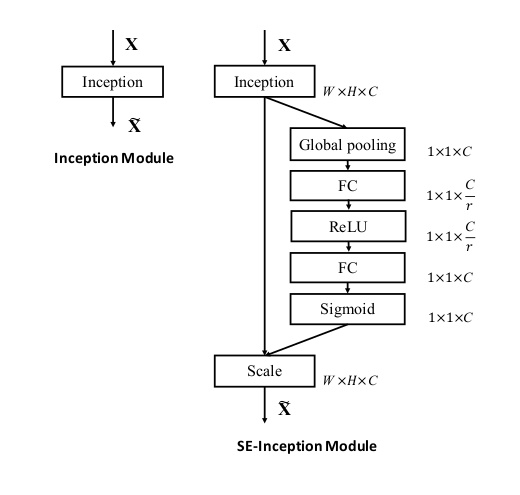
\includegraphics[width=0.45\textwidth]{DLTips/SEInception0.jpg}
}
\:
\subfigure[SE-ResNet Module]{\label{SEResNet0}
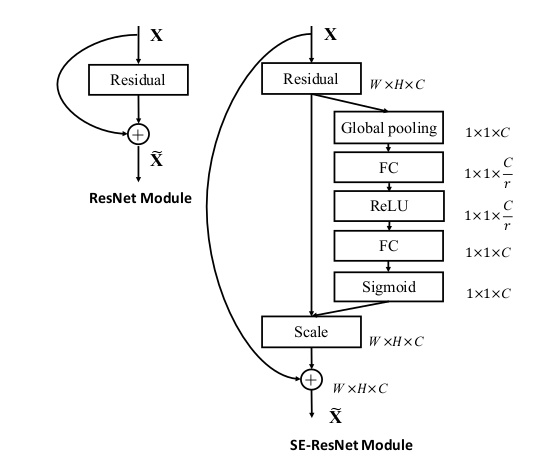
\includegraphics[width=0.45\textwidth]{DLTips/SEResNet0}
}
\caption{SENet与Inception以及ResNet结合的示意图}
\label{SENetConv1}
\end{figure}

\subsection{小结-比较}

图\ref{Conv0}是对上面提到的不同的卷及类型的一个比较与总结。

\begin{figure}
\centering
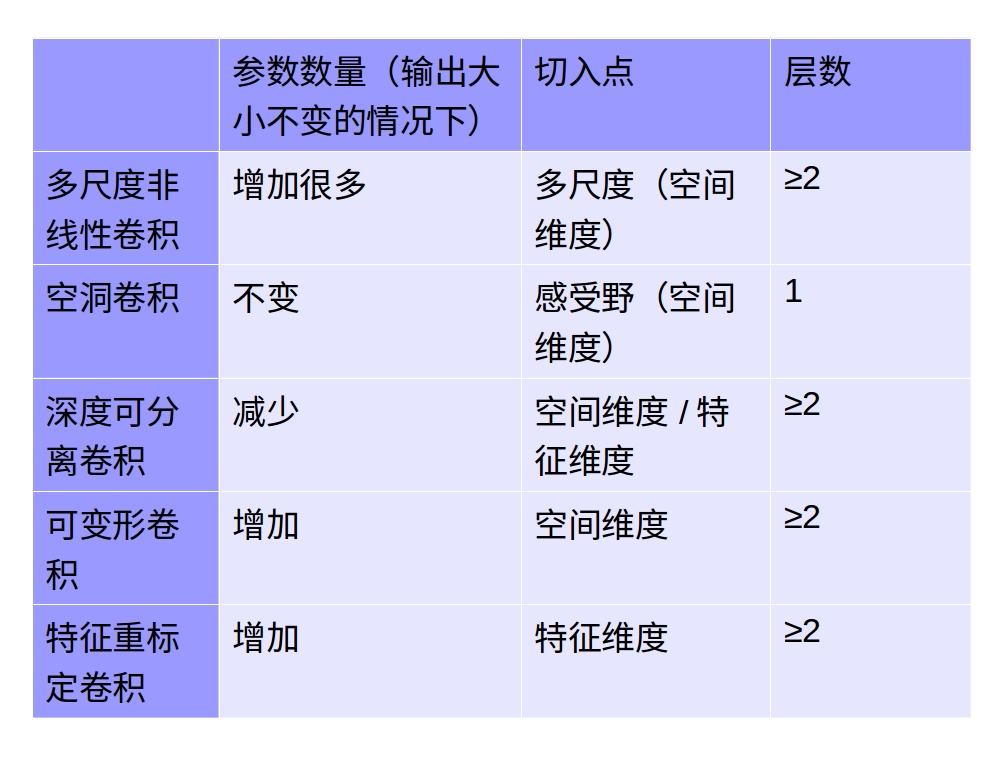
\includegraphics[width=0.75\textwidth]{DLTips/Conv0.jpg}
\caption{不同卷积策略的比较}
\label{Conv0}
\end{figure}

我们把图像(height,width)作为空间维度,把channels做为特征维度。

\section{全连接与卷积的异同}
全连接:Fully Connected

注意这里与FCN中的FC不同,FCN里面的FC是Fully Convolution,所以还是卷积操作,所以才有用Fully Convolution代替Fully Connected之说。

Fully Connected的作用是什么?其本质上还是一个卷积运算,只不过输入卷积核的大小跟最后一层Feature Map的大小一致, 所以得到的结果是一个标量。其实就是对前面CNN网络提取的特征进行变换,对这些Feature maps进行组合,得到目标类的一个代表值,输入Sigmoid函数进行计算,得到分类结果。但这种方式参数非常多,因为在实现Fully Connected时需要根据最后一层Feature Map的大小来确定计算的卷积核,这也导致了它需要解决不同输入大小时候的数据问题。

一个简单的例子,输入是$228 * 228 * 3$,然后最后一层Feature Map的维度是$7 * 7 * 512$,即,共包含512个Feature Maps,每一个Feature Map的大小是$7 * 7$,那么全连接层需要这样设计,假设我们想要输出1024个分类,那么全连接的参数的数量就是:
$7 * 7 * 512 * 1024$,所以参数非常多!另一方面,如果输入不是$228 * 228 * 3$而是$456 * 456 * 3$那么,得到的最后一层Feature map的大小也不是$7 * 7 * 512$,现在而是$14 * 14 * 512$,那么全连接也需要改变,变成$14 * 14 * 512 * 1024$, 这样非常不灵活。

因为参数实在太多,所以现在在最后为了得到Sigmoid函数的输入(标量),都选择使用Global Average Pooling来代替全连接。Global Average Pooling也就是说用一个Feature Map的平均值作为Sigmoid输入,输出为类别信息。

不过,也有研究人员表明,全连接层有助于在微调(Fine-tune)过程中进行知识迁移,尤其源领域与目标领域很不一样的时候,更是如此。

\section{Pooling}

\subsubsection{Global Average Pooling}

就是对一个Feature Map进行加和求平均值。具体的应用可参考上一小节。

\subsubsection{Unpooling}

而上池化的实现主要在于池化时记住输出值的位置,在上池化时再将这个值填回原来的位置,其他位置填0即OK。(参考:SegNet, DeconvNet)

\begin{figure}[!hbtp]
\centering
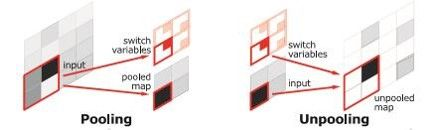
\includegraphics[width=0.75\textwidth]{DLTips/Unpooling0.png}
\caption{Unpooling示意图}
\label{Unpooling0}
\end{figure}

图\ref{Unpooling0}可以认为额外的\verb|switch variables|实现了保存Pooling过程中的位置。

In the convnet, the max pooling operation is non-invertible, however we can obtain an approximate inverse by recording the locations of the maxima within each pooling region in a set of switch variables. In the deconvnet, the unpooling operation uses these switches to place the reconstructions from the layer above into appropriate locations, preserving the structure of the stimulus.

也就是说用一组开关变量保存最大值在Pooling Region中的位置。

参考文献: \href{https://www.quora.com/What-is-the-difference-between-Deconvolution-Upsampling-Unpooling-and-Convolutional-Sparse-Coding}{Quora Answer}

\section{Local Response Normalization}

Reference: \href{https://prateekvjoshi.com/2016/04/05/what-is-local-response-normalization-in-convolutional-neural-networks/}{What is LRN}

为什么需要设置Normalization Layers?
Anyway, the reason we may want to have normalization layers in our CNN is that we want to have some kind of inhibition scheme. 这个Inhibition Scheme是什么意思。

侧边抑制:ateral inhibition。 一个激活的神经会抑制旁边神经的激活。

\subsubsection{到底什么是LRN}

Local Response Normalization (LRN) layer implements the lateral inhibition we were talking about in the previous section. This layer is useful when we are dealing with ReLU neurons. Why is that? Because ReLU neurons have unbounded activations and we need LRN to normalize that. We want to detect high frequency features with a large response. If we normalize around the local neighborhood of the excited neuron, it becomes even more sensitive as compared to its neighbors.

At the same time, it will dampen(抑制) the responses that are uniformly large in any given local neighborhood(值普遍很大的局部). If all the values are large, then normalizing those values will diminish all of them. So basically we want to encourage some kind of inhibition and boost the neurons with relatively larger activations. 

\subsubsection{如何实现LRN}

There are two types of normalizations available in Caffe. You can either normalize within the same channel or you can normalize across channels. Both these methods tend to amplify the excited neuron while dampening the surrounding neurons. When you are normalizing within the same channel, it’s just like considering a 2D neighborhood of dimension N x N, where N is the size of the normalization window. You normalize this window using the values in this neighborhood. If you are normalizing across channels, you will consider a neighborhood along the third dimension but at a single location. You need to consider an area of shape N x 1 x 1. Here 1 x 1 refers to a single value in a 2D matrix and N refers to the normalization size.

在 AlexNet 中Normalized的计算公式如下:

\begin{displaymath}
b_{x, y}^i = a_{x, y}^i / \left( k + \alpha \sum_{j = \max(0, i - n/2)}^{\min(N-1, i + n/2)(a_{x, y}^j)^2} \right)
\end{displaymath}

其中, $a_{x, y}^i, b_{x, y}^i$分别是输入的激活值,输出的Normalized的值。

\section{CNN中感受野的计算}

参考文献:

[1] \href{https://blog.csdn.net/kuaitoukid/article/details/46829355}{CNN中感受野的计算-CSDN}

[2] \href{https://www.cnblogs.com/objectDetect/p/5947169.html}{CNn中感受野的计算-博客园}

感受野(receptive field)是怎样一个东西呢,从CNN可视化的角度来讲,就是输出featuremap某个节点的响应对应的输入图像的区域就是感受野。

比如我们第一层是一个3*3的卷积核,那么我们经过这个卷积核得到的featuremap中的每个节点都源自这个3*3的卷积核与原图像中3*3的区域做卷积,那么我们就称这个featuremap的节点感受野大小为3*3

如果再经过pooling层,假定卷积层的stride是1,pooling层大小2*2,stride是2,那么pooling层节点的感受野就是4*4

有几点需要注意的是,padding并不影响感受野,stride只影响下一层featuremap的感受野,size影响的是该层的感受野。

具体计算时,需要:
\begin{itemize}
\item 第一层卷积层的输出特征像素的感受野的大小就是滤波器的大小
\item 深层卷积层的感受野大小和它之前的所有层的滤波器大小和步长有关系
\item 计算感受野大小时,忽略图像边缘的影响,即不考虑Padding的大小。
\end{itemize}

关于感受野的计算,多采用Top to Down的方式,即最先计算最深层的前一层的感受野,然后逐渐传递到第一层,使用的公式如下:
\begin{enumerate}
\item RF = 1   // 待计算的Feature Map的感受野大小
\item For layer in (top layer to down layer):
\item      RF = ((RF - 1) * stride) + fsize
\end{enumerate}

stride 表示卷积的步长; fsize表示卷积层滤波器的大小。

\subsubsection{具体的例子}

%\begin{table}
\begin{tabular}{ccc}
\toprule
type & size & stride \\
\midrule
conv1 & 3 & 2 \\
pool1 & 2 & 2 \\
conv2 & 3 & 1 \\
pool2 & 2 & 2 \\
conv3 & 3 & 1 \\
conv4 & 3 & 1 \\
pool3 & 2 & 2 \\
\bottomrule
\end{tabular}
%\end{table}

pool3的一个输出对应pool3的输入大小为2*2

感受野计算如下:

依次类推,对应conv4的输入为4*4,因为2*2的每个角加一个3*3的卷积核,就成了4*4,当然这是在stride=1的情况下才成立的,但是一般都是stride=1,不然也不合理

对应conv3的输入为6*6

对应pool2的输入为12*12

对应conv2的输入为14*14

对应pool1的输入为28*28

对应conv1的输入为30*30

所以pool3的感受野大小就是30*30

\subsubsection{Stride的计算}

每一个卷积层有一个Strides的概念,这个Strides就是之前所有层Stride的乘积。即
\begin{displaymath}
strids(i) = stride(1) * stride(2) * stride(3) * \ldots * stride(i - 1)
\end{displaymath}

\subsubsection{专业的计算}

参考文献:\href{https://zhuanlan.zhihu.com/p/26663577}{卷积神经网络中的感受野计算(译)-知乎}, \href{https://medium.com/mlreview/a-guide-to-receptive-field-arithmetic-for-convolutional-neural-networks-e0f514068807}{原文-英语}

定义:The receptive field is defined as the region in the input space that a particular CNN’s feature is looking at (i.e. be affected by).

这篇英语文章,主要是四个公式:
\begin{itemize}
\item Calculate the number of output features

\begin{displaymath}
n_{out} =	\lfloor \frac{n_{in} + 2p - k}{s} \rfloor + 1
\end{displaymath}

其中,$p$表示单侧Padding大小, $k$表示filter kernel的大小。


\item Calculate the Jump (Strides) in the output feature map

\begin{displaymath}
j_{out} = j_{in} * s
\end{displaymath}

其中, $j$表示Strides,注意stride是不断积累的。如上下文中提到的。

\item Calculate the receptive field size

\begin{displaymath}
r_{out} = r_{in} + (k - 1) * j_{in}
\end{displaymath}

$k$表示kernel filter的大小。

\item Calculate the center position of the receptive field of the first output feature

\begin{displaymath}
start_{out} = start_{in} + (\frac{k - 1}{2} - p) * j_{in}
\end{displaymath}

\end{itemize}

The first layer is the input layer, which always has n = image size, r = 1, j = 1, and start = 0.5. 

小结如图\ref{PerceptionField1}所示。
\begin{figure}[!htbp]
\centering
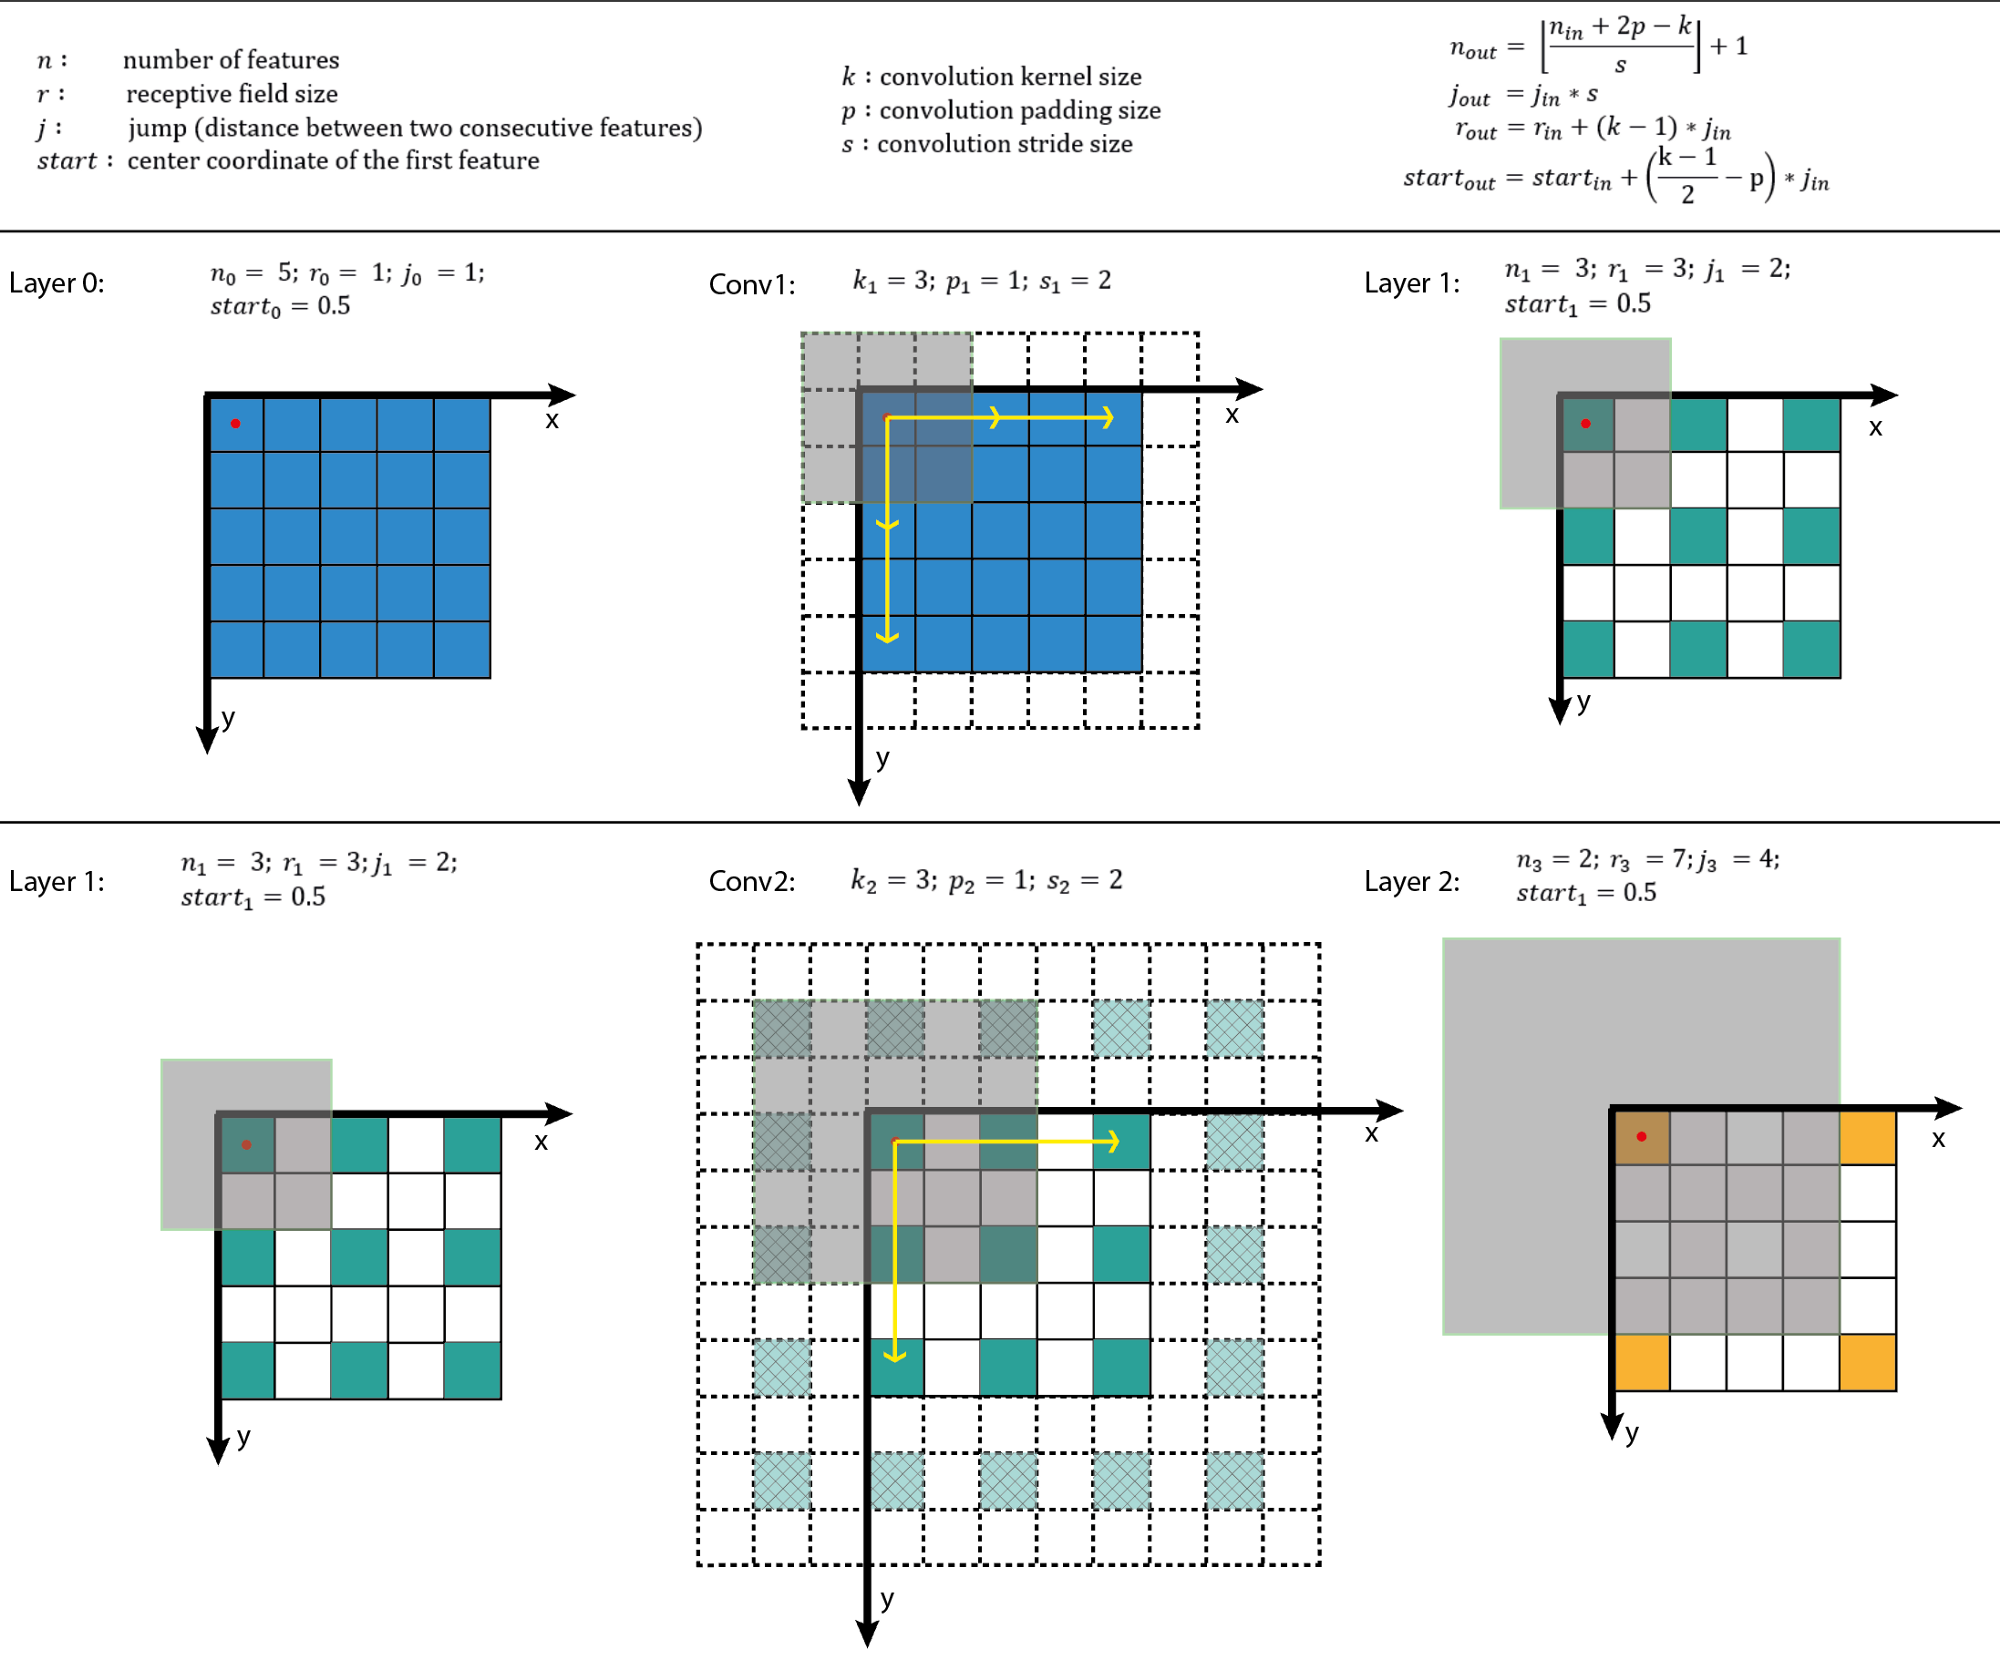
\includegraphics[width=0.8\textwidth]{DLTips/PerceptionField1.png}
\caption{文章的总结与说明}
\label{PerceptionField1}
\end{figure}


\href{https://zhuanlan.zhihu.com/p/28492837}{神经网络中的感受野-知乎}

由于图像是二维的,具有空间信息,因此感受野的实质其实也是一个二维区域。但业界通常将感受野定义为一个正方形区域,因此也就使用边长来描述其大小了。在接下来的讨论中,本文也只考虑宽度一个方向。我们先按照图\ref{PerceptionField0}所示对输入图像的像素进行编号。

\begin{figure}[!hbtp]
\centering
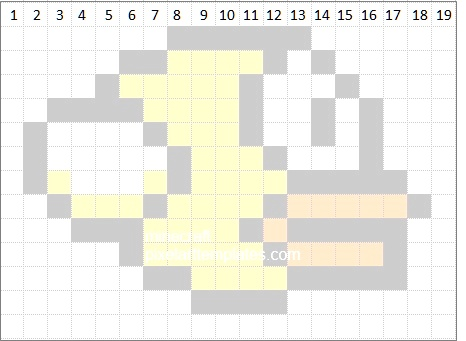
\includegraphics[width=0.75\textwidth]{DLTips/PerceptionField0.jpg}
\caption{二维图像像素编号示意图}
\label{PerceptionField0}
\end{figure}

接下来我们使用一种并不常见的方式来展示CNN的层与层之间的关系(如下图,请将脑袋向左倒45°观看$>\_<$),并且配上我们对原图像的编号。

图中黑色的数字所构成的层为原图像或者是卷积层,数字表示某单元能够看到的原始图像像素。我们用 $r_n$ 来表示第 n 个卷积层中,每个单元的感受野(即数字序列的长度);蓝色的部分表示卷积操作,用 $k_n$ 和 $s_n$ 分别表示第 n 个卷积层的kernel\_size和stride。

对Raw Image进行kernel\_size=3, stride 2的卷积操作所得到的fmap1 (fmap为feature map的简称,为每一个conv层所产生的输出)的结果是显而易见的。序列[1 2 3]表示fmap1的第一个单元能看见原图像中的1,2,3这三个像素,而第二个单元则能看见3,4,5。这两个单元随后又被kernel\_size=2,stride 1的Filter 2进行卷积,因而得到的fmap2的第一个单元能够看见原图像中的1,2,3,4,5共5个像素(即取[1 2 3]和[3 4 5]的并集)。

接下来我们尝试一下如何用公式来表述上述过程。可以看到,[1 2 3]和[3 4 5]之间因为Filter 1的stride 2而错开(偏移)了两位,而3是重叠的。对于卷积两个感受野为3的上层单元,下一层最大能获得的感受野为 $3\times2=6$ ,但因为有重叠,因此要减去(kernel\_size - 1)个重叠部分,而重叠部分的计算方式则为感受野减去前面所说的偏移量,这里是2. 因此我们就得到 $r_2=r_1\times k_2-(r_1-s_1)\times(k_2-1)=3\times2-(3-2)\times(2-1)=5$ 。

继续往下一层看,我们会发现[1 2 3 4 5]和[3 4 5 6 7]的偏移量仍为2,并不简单地等于上一层的 $s_2$ ,\textbf{这是因为之前的stride对后续层的影响是永久性的},而且是累积相乘的关系(例如,在fmap3中,偏移量已经累积到4了),也就是说 $r_3$ 应该这样求 

\begin{displaymath}
r_3=r_2\times k_3-(r_2-s_1\times s_2)\times(k_3-1)=5\times3-(5-2)\times(3-1)=9 
\end{displaymath}

以此类推,

\begin{displaymath}
r_4=r_3\times k_4-(r_3-s_1\times s_2\times s_3)\times(k_4-1)=9\times2-(9-4)\times(2-1)=13 
\end{displaymath}


于是我们就可以得到关于计算感受野的抽象公式了: 

\begin{displaymath}
r_n=r_{n-1}\times k_n-(r_{n-1}-\prod_{i=1}^{n-1}s_i)\times(k_n-1) 
\end{displaymath}


经过简单的代数变换之后,最终形式为:

\begin{displaymath}
r_n=r_{n-1}+(k_n-1)\prod_{i=1}^{n-1}s_i 
\end{displaymath}

这个公式也体现了上文提到的stride影响的下一层。


\section{神经网络中的初始化}

\subsubsection{回答一}

参考文献:\href{https://www.zhihu.com/question/56526007}{为什么要进行初始化-知乎}

参数初始化的目的是为了让神经网络在训练过程中学习到有用的信息,这意味着参数梯度不应该为0。所以参数初始化应该满足两个条件:
\begin{itemize}
\item 各个激活层不会出现饱和现象,比如对于Sigmoid激活函数,初始化值不能太大也不能太小,导致进入饱和区
\item 各个激活值不为0,如果激活层输出为0,也就是下一层的输入为0, 所以这个卷积层对权重的偏导数为0, 那么导致梯度也为0
\item 另一个非常重要的原因,就是Xavier, MSRA等这些初始化不至于一开始就让网络发散,或者梯度消失
\end{itemize}

所以,最主要要注意两个问题,首先是梯度不能消失,然后网络不能发散。

\subsection{Xavier}

参考文章:\href{https://zhuanlan.zhihu.com/p/27919794}{深度前馈网络与Xavier初始化原理-知乎}

而为什么把模型的参数初始化成全0就不行了呢?这个不用讲啦,全0的时候每个神经元的输入和输出没有任何的差异,换句话说,根据前面BP算法的讲解,这样会导致误差根本无法从后一层往前传(乘以全0的$\omega$后误差就没了),这样的model当然没有任何意义。

{\bfseries 那么我们不把参数初始化成全0,那我们该初始化成什么呢?换句话说,如何既保证输入输出的差异性,又能让model稳定而快速的收敛呢?}

要描述“差异性”,首先就能想到概率统计中的方差这个基本统计量。对于每个神经元的输入z这个随机变量,根据前面讲BP时的公式,它是由线性映射函数得到的,也就是:
\begin{displaymath}
z = \sum_{i = 1}^{n}\omega_i x_i
\end{displaymath}

其中n是上一层神经元的数量。因此,根据概率统计里的两个随机变量乘积的方差展开式

\begin{displaymath}
Var(\omega_i x_i) = E[\omega_i]^2 Var(x_i) + E[x_i]^2Var(\omega_i) + Var(\omega_i)Var(x_i)
\end{displaymath}

所以,如果$E(x_i) = E(\omega_i)=0$(可以通过批量归一化Batch Normlization来满足,其它大部分情况也不会差太多), 那么就有:
\begin{displaymath}
Var(z) = \sum_{i = 1}^{n}Var(x_i)Var(\omega_i)
\end{displaymath}

如果变量$x_i$与$\omega_i$满足独立同分布的话:
\begin{displaymath}
Var(z) = n \cdot Var(x)Var(\omega)
\end{displaymath}

好了,这时重点来了。试想一下,根据文章《激活函数》,整个大型前馈神经网络无非就是一个超级大映射,将原始样本稳定的映射成它的类别。也就是将样本空间映射到类别空间。试想,如果样本空间与类别空间的分布差异很大,比如说类别空间特别稠密,样本空间特别稀疏辽阔,那么在类别空间得到的用于反向传播的误差丢给样本空间后简直变得微不足道,也就是会导致模型的训练非常缓慢。同样,如果类别空间特别稀疏,样本空间特别稠密,那么在类别空间算出来的误差丢给样本空间后简直是爆炸般的存在,即导致模型发散震荡,无法收敛。因此,我们要让样本空间与类别空间的分布差异(密度差别)不要太大,也就是要让它们的方差尽可能相等。这里的样本空间与类别空间可以理解成是输入$x$空间与输出$z$的空间,以及其所对应的方差。

如果需要两个空间的方差差异不大,即满足$Var(z) = Var(x)$, 那么需要$n \cdot \omega = 1$, 也就是说$Var(\omega) = 1 / n$。其中$n$表示神经元输出端对应的个数。在前向传播时,对于特定一层神经网络,$n = n_{in}$, 在后向传播时,$n = n_{out}$而一般这两者都不相同,因此可以取它们的中间值:
\begin{displaymath}
Var(\omega) = \frac{1}{\frac{n_{in} + n_{out}}{2}}
\end{displaymath}

假设$\omega$均匀分布时,由$\omega$在区间$[a, b]$内均匀分布的方差为:
\begin{displaymath}
Var = \frac{(b - a)^2}{12}
\end{displaymath}

联立上面两个公式,可以得出$\omega$的分布区间(假设$b = -a$):
\begin{displaymath}
\omega \sim U\left[ -\frac{\sqrt{6}}{\sqrt{n_{in} + n_{out}}}, \frac{\sqrt{6}}{\sqrt{n_{in} + n_{out}}}  \right]
\end{displaymath}
(让w在这个区间里均匀采样就好啦)

得到的这个结论就是Xavier初始化方法。这就是为什么使用Xavier初始化这个trick经常可以让model的训练速度和分类性能取得大幅提高啦~所以在使用前馈网络时,除非你的网络设计的明显不满足xavier的假设,否则使用xavier往往不会出错。当然,另一方面来说,也很少有场合可以完全迎合xavier假设,因此时间充裕的话,改改分子,甚至去掉$n_{out}$都有可能带来意想不到的效果。


\section{计算图的后向传播计算}

参考文章:

[1] \href{https://zhuanlan.zhihu.com/p/27919794}{深度前馈网络与Xavier初始化原理-知乎}

[2] \href{https://mp.weixin.qq.com/s?__biz=MzIwNzc2NTk0NQ==&mid=2247484344&idx=1&sn=92ff388d93088ea6461023b376860ce7&chksm=970c2b6ea07ba2782da5de78b23b78b267b4b0fc4454e76256134cfc9d6aa5416e0bd4c14097&scene=21#wechat_redirect}{BP算法-夕小瑶}

\subsubsection{简单的说明}
误差反向传播过程, 其本质就是基于链式求导 + 梯度下降。

首先往上翻一翻,记住之前说过的前馈网络无非就是反复的线性与非线性映射。

首先,假设某个神经元的输入为z,经过激活函数$f_1(\cdot)$得到输出a。即函数值$a=f_1(z)$。如果这里的输入z又是另一个函数f2的输出的话(当然啦,这里的$f_2$就是线性映射函数,也就是连接某两层的权重矩阵),即$z=f_2(x)$,那么如果基于a来对z中的变量x求导的时候,由于 

\begin{displaymath}
\frac{\partial a}{\partial x} = \frac{\partial a}{\partial z}\cdot \frac{\partial z}{\partial x} = f_1^{'}(z)\frac{\partial z}{\partial x}
\end{displaymath}

上式也就是链式求导。更一般的链式求导法则为:
\begin{displaymath}
\frac{\partial a}{\partial x} = \sum_{i} \frac{\partial a}{\partial z_i}\cdot \frac{\partial z_i}{\partial x}
\end{displaymath}

显然只要乘以激活函数f1的导数,就不用操心激活函数的输出以及更后面的事儿了(这里的“后面”指的是神经网络的输出端方向),只需要将精力集中在前面的东西,即只需要关注z以及z之前的那些变量和函数就可以了。因此,误差反向传播到某非线性映射层的输出时,只需要乘上该非线性映射函数在z点的导数就算跨过这一层啦。

而由于$f2(\cdot)$是个线性映射函数,即 $f_2(x)=\omega \cdot x + b$,因此
\begin{displaymath}
\frac{\partial z}{\partial x} = \omega
\end{displaymath}
因此,当误差反向传播到线性映射层的输出时,若想跨过该层,只需要乘以线性映射函数的参数就可以啦~即乘上$\omega$。

而这里的x,又是更前面的非线性映射层的输出,因此误差在深度前馈网络中反向传播时,无非就是反复的跨过非线性层和线性层,也就是反复的乘以非线性函数的导数(即激活函数的导数)和线性函数的导数(即神经网络的参数/权重/连接边)。

也就是下面这张图啦(从右往左看):

\begin{figure}[!bthp]
\centering
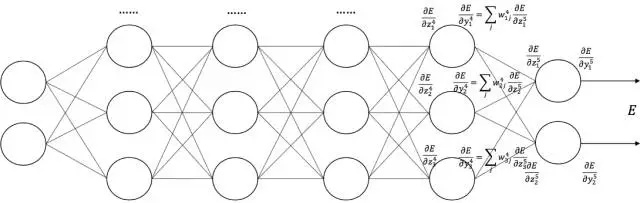
\includegraphics[width=0.75\textwidth]{DLTips/BP0.jpg}
\caption{BP计算过程示意图}
\label{BP0}
\end{figure}

\section{神经网络中的Attention机制}

参考文献:\href{https://zhuanlan.zhihu.com/p/35571412}{浅谈Attention机制-知乎}

\subsection{Recurrent Models of Visual Attention}

参考文献:\cite{Attention2014}

Our model considers attention-based processing of a visual scene as a control problem and is general enough to be applied to static images, videos,
or as a perceptual module of an agent that interacts with a dynamic visual environment (e.g. robots,
computer game playing agents).

Instead of processing an entire image or even bounding box at once, at each step, the model
selects the next location to attend to based on past information and the demands of the task.

We describe an end-to-end
optimization procedure that allows the model to be trained directly with respect to a given task and
to maximize a performance measure which may depend on the entire sequence of decisions made by
the model. This procedure uses backpropagation to train the neural-network components and policy
gradient to address the non-differentiabilities due to the control problem

目标检测的几种方法:
\begin{itemize}
\item 基于窗口的分类器,包括Proposal等, 计算量大
\item 基于Saliency Detection的, 不能Interate information across fixations, 仅利用底层图像特征, 忽略了Semantic Content of a scene and task demands.
\item 一些工作把视觉问题当做Sequential decision task,本文也是
\item 
\end{itemize}

Our formulation which employs an RNN to integrate visual
information over time and to decide how to act is, however, more general, and our learning procedure
allows for end-to-end optimization of the sequential decision process instead of relying on greedy
action selection.

我们的模型,既可以实现性质图像的Object Recognition, 而且还适用于动态环境,以一种Task-driven的方式。

\subsubsection{The Recurrent Attention Model - RAM }

In this paper we consider the attention problem as the sequential decision process of a goal-directed
agent interacting with a visual environment.

这篇文章里面,感觉这意思,Attention机制不就是Reinforcement Learning么?

该公式包含了各种任务,如静态图像中的对象检测, 控制问题,即根据屏幕上的图像流来学习打游戏等。

\begin{figure}[!htbp]
\centering
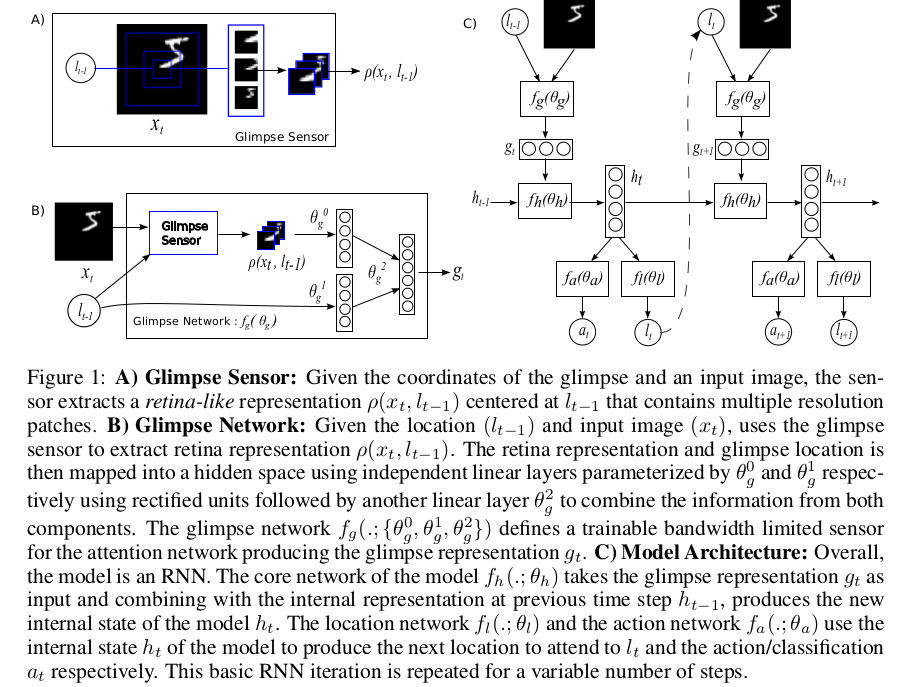
\includegraphics[width=0.75\textwidth]{DLTips/Attention0.png}
\caption{Attention 模型示意图}
\label{Attention0}
\end{figure}

图\ref{Attention0}中,$x_t$表示第$t$时刻的输入图像,$l_{t-1}$表示位置,$\rho (x_t, l_{t-1})$表示这个位置的Retina-like representation. $g_t$为glimpse representation。 

We will refer to this low-resolution representation
as a glimpse。

Action分为两个部分:
\begin{itemize}
\item Location actions

are chosen stochastically from a distribution parameterized by the location network $f_l(h_t; \theta_t)$ at time $t$。

\item Environment action

The environment action a t is similarly drawn from a distribution conditioned
on a second network output $a_t \sim p(\cdot | f_a(h_t; \theta_a))$

\end{itemize}

与RL里面的Partially Observable Decision Process (POMDP)的一个特例。

\subsubsection{总结}

感觉本文中的Attention与RL关系密切,而且与RNN网络结合起来了。那么到底什么是Attention机制,还需要阅读其它文章,现在我还不太明白。


\section{小型网络}

参考文章:\href{https://zhuanlan.zhihu.com/p/37074222}{CVPR2018高效小网络-知乎}

\subsection{理论分析}

先说结论:卷积层主要引入了计算量,全连接层主要引入了参数数量。

参数数量用params表示,关系到模型大小,单位通常为M,通常参数用float32表示,所以模型大小是参数数量的4倍。

理论计算量用FLOPs或者M-Adds表示,这里用FLOPs写起来简单,关系到算法速度,大模型的单位通常为G,小模型通道为M。

需要注意的两点:
\begin{itemize}
\item 理论计算量通常只考虑乘加操作(Multi-Adds)的数量,而且只考虑CONV和FC等参数层的计算量,忽略BatchNorm和PReLU等等。一般情况,CONV和FC层也会忽略仅纯加操作的计算量,如bias偏置加和shotcut残差加等,\textbf{目前技术有BN的CNN可以不加bias}。

\item 理论计算量通常和实际ARM实测速度会有不一致,主要是理论计算量太过理论化,没有考虑不同硬件IO速度和计算力差异,最重要的是inference framework部署框架优化水平和程度差异,不同框架的优化的关注点不一样,同一框架对不同层的优化程度也不一样。Inference Framework以我用过的ncnn为代表。
\end{itemize}

假设,卷积核大小为$k_h * k_w$, 输入的特征的通道为$C_{in}$,输出的Feature Map的数量为$C_{out}$, Feature Map的尺寸是$H*W$。那么,\textbf{卷积层}对应的参数量\textit{params}和计算量\textit{FLOPs}分别是:

\begin{displaymath}
\begin{gathered}
\#Params: (k_h * k_w * c_{in} + 1) * c_{out} \\
\#FLOPs: k_w * k_h * c_{in} * c_{out} * W * H
\end{gathered}
\end{displaymath}

相对比的,\textbf{全连接层}对应的上述两个参数分别是:
\begin{displaymath}
\begin{gathered}
\#Params: (c_{in} + 1) * C_{out} \\
\#FLOPs: c_{in} * c_{out}
\end{gathered}
\end{displaymath}

\subsection{GCONV \& DWCONV}

有时间在整理吧,细节见原文。

结论就是,通过输入通道的分组,可以降低参数量以及计算量$g$倍,其中$g$是输入通道的分组数,并且在DWCONV中这个分组数$g$就是输入的通道数$C_{in}$。

其它的一点说明:

设计CNN目前都采用堆block的方式,后面对每个模型只集中分析其block的设计。堆Block简化了网络设计问题:只要设计好block结构,对于典型224 $\times$ 224输入,设计CNN只需要考虑112$\times$112、56$\times$56、28$\times$28、14$\times$14、7$\times$7 这5个分辨率阶段(stage)的block数量和通道数量就可以了。

CNN加深度一般都选择14$\times$14这个分辨率阶段,多堆几个block,这一层的参数数量和计算量占比最大,所以我们选这一层作为特例分析每种block的参数数量和计算量,量化说明选择$14\times14\times512$的输入和输出情况。

\subsection{NiN及相关}




\section{Deep Reinforcement Learning}

参考文献:\href{https://deeplearning4j.org/deepreinforcementlearning}{A Beginner's Guide to Deep Reinforcement Learning}

几个重要的摘抄。
\begin{itemize}
\item Algorithms can start from a blank slate, and under the right conditions they achieve superhuman performance. Like a child incentivized by spankings and candy, these algorithms are penalized when they make the wrong decisions and rewarded when they make the right ones – this is reinforcement.

\item Reinforcement learning solves the difficult problem of correlating immediate actions with the delayed returns they produce. 
\end{itemize}

\section{为什么Python中要继承object类}

参考文章:\href{https://stackoverflow.com/questions/4015417/python-class-inherits-object}{stackoverflow answer}

在Python3中,除了因为要兼容于Python2,没有其它原因。而在Python2中,则有些复杂。

\subsubsection{Python 2.x story}
Python2(从python2.2开始)中,有两种类型的类(two styles of classes), 他们根据是否继承自\textbf{object}来区分。

\begin{itemize}
\item Classic style classes, they don't have object as a base class
\item New style classes: they have, directly or indirectly (\textit{e.g.} inherit from a built-in type), \textbf{object} as a base class
\end{itemize}

那么为什么选择用新式类呢(New style classes)?几个原因如下:
\begin{itemize}
\item Support for descriptors. Sepcifically, the following constructs are made possible with descriptors:
\begin{itemize}
\item classmethod
\item staticmethod
\item properties with property
\item \_\_slots\_\_
\end{itemize}
\item the \verb|__new__| static method
\item method resolution order (MRO)
\item Related to MRO
\end{itemize}

\subsubsection{Python 3.x story}

In Python 3, things are simplified. Only new-style classes exist (referred to plainly as classes) so, the only difference in adding object is requiring you to type in 8 more characters. 


\subsubsection{Choose which one}

\begin{itemize}
\item \textbf{In Python 2.x}, \textbf{always} inherit from \textbf{object} explicitly
\item \textbf{In Python 3.x}, inherit \textbf{object} if you are writing code that tries to be Python agnostic (不可知论者), that is, it needs to work both in python 2 and in python 3. Otherwise, don't, it really makes no difference since Python inserts it for you behind the scenes.
\end{itemize}

\section{1*1卷积}

参考文章:\href{https://www.zhihu.com/question/56024942}{1*1卷积的作用与好处-知乎}

1*1卷积 和正常的卷积一样,唯一不同的是它的大小是1*1,没有考虑在前一层局部信息之间的关系, 所以这里跟普通说卷积的时候一样,都是自动忽略了在Channel上的维度,而只是空间域的维度是1*1或3*3或5*5等。最早出现在 Network In Network的论文中 ,使用1*1卷积是想加深加宽网络结构 ,在Inception网络( Going Deeper with Convolutions )中用来降维,

由于3*3卷积或者5*5卷积在几百个filter的卷积层上做卷积操作时相当耗时,所以1*1卷积在3*3卷积或者5*5卷积计算之前先降低维度。(说的是Channel的维度。)

所以1*1卷积的主要作用有以下几点:
\begin{itemize}
\item 降维

比如,一张500 * 500且厚度depth为100 的图片在20个filter上做1*1的卷积,那么结果的大小为500*500*20。

\item 加入非线性

卷积层之后经过激励层,1*1的卷积在前一层的学习表示上添加了非线性激励( non-linear activation ),提升网络的表达能力。类似于在一个像素位置,在所有Channel上进行非线性变换,而不考虑附近的信息。

\end{itemize}

所以1*1卷积实际上是对每个像素点,在不同的Channel上进行线性组合, 即信息整合,且保留图像的原有平面结构,调控Depth, 自动完成升维、降维的作用。如下图所示,如果选择2个filter的1*1,那么数据就从原来的depth为3变为depth为2.若用4个filter,则起到了升维的作用。
\begin{figure}[!hbtp]
\centering
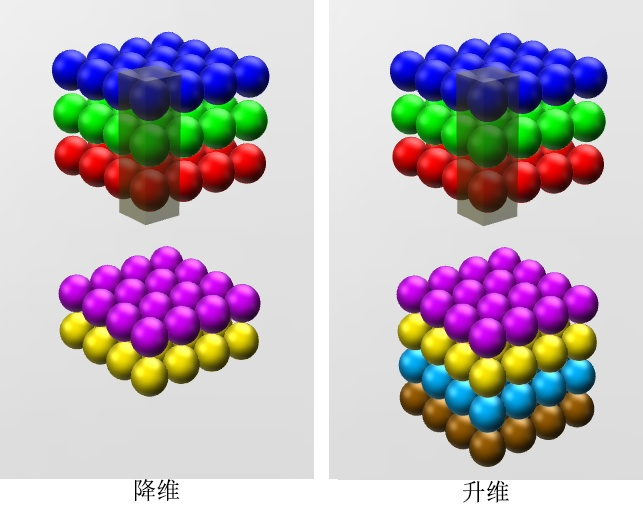
\includegraphics[width=0.75\textwidth]{DLTips/OneOneConv0.jpg}
\caption{1*1 Convolutoin 的作用示意图}
\label{OneOneConv0}
\end{figure}

\section{目标检测中完整流程}

由于几个经典的目标检测模型的实现不是很复杂,所以这里主要记录数据的处理过程。首先输入是什么数据、用到了哪些增广技术、输入图像的尺寸、输出是什么形式、目标函数怎么实现怎么优化、怎么评估结果等等。

在目标检测中,主要用到的评估指标是:mAP、IOU。但是怎么实现呢?

目标函数是什么,如何实现BBox的确定等等,好麻烦啊。




\section{待续}













